\documentclass[a4paper]{article}
\usepackage[utf8]{inputenc}
\usepackage[english]{babel}
\usepackage{csquotes}
\usepackage{amsmath} % per ambienti tipo cases
\usepackage{amssymb}
\usepackage{mathtools}
\usepackage{siunitx}
\usepackage{graphicx} % per includere figure
%\usepackage{subfigure}
\usepackage{booktabs} % per le tabelle
\usepackage{caption}
\usepackage{fancyhdr}
\usepackage{hyperref}
\usepackage[section]{placeins}
\usepackage{microtype}
\usepackage{caption}
\usepackage{subcaption}
\captionsetup[subfigure]{labelfont=rm}
\usepackage{verbatim} %multiline comments
\usepackage{wrapfig}
\usepackage[backend=biber, style=numeric, safeinputenc, sorting=none]{biblatex}
\addbibresource{source.bib}	% uncomment for bibliography



%opening
\title{}
\author{}

\pagestyle{fancy}
\lhead{Musical Acoustics}
\chead{H6}
\rhead{10743504, 10751919}
\newcommand{\Rarrow}{\mbox{\Large$\Rightarrow$}}

\begin{document}

\begin{titlepage}	
	\newcommand{\HRule}{\rule{\linewidth}{0.5mm}} % Defines a new command for horizontal lines, change thickness here
	
	\center % Centre everything on the page
	
	%------------------------------------------------
	%	Headings
	%------------------------------------------------
	
	
\includegraphics[width=.4\textwidth]{Logo_Politecnico_Milano.png}\\[0.4cm]
	\textsc{\LARGE}\\[0.3cm] % Main heading such as the name of your university/college
	
	\textsc{\large MSc. Music and Acoustic Engineering}\\[1cm] % Minor heading such as course title
	
	\textsc{\Large Musical Acoustics - A.Y. 2020/2021}\\[0.5cm] % Major heading such as course name
	
	%------------------------------------------------
	%	Title
	%------------------------------------------------
	
	\HRule\\[0.4cm]
	
	{\huge\bfseries H6 - Design of a Recorder Flute }\\[0.4cm] % Title of your document
	
	\HRule\\[1.5cm]
	
	
	
	{\large\textit{Authors' IDs:}}\\
	10743504, 10751919, % Your name
	%\\ \textsc{Gruppo 11}
	
	%------------------------------------------------
	%	Date
	%------------------------------------------------
	
	\vfill\vfill\vfill % Position the date 3/4 down the remaining page
	
	{\large\today} % Date, change the \today to a set date if you want to be precise
	
	%------------------------------------------------
	%	Logo
	%------------------------------------------------
	
	\vfill\vfill
	%\includegraphics[width=0.2\textwidth]{Politecnico_di_Milano.eps}\\[1cm] % Include a department/university logo - this will require the graphicx package
	
	%----------------------------------------------------------------------------------------
	
	\vfill % Push the date up 1/4 of the remaining page
	
	
\end{titlepage}

\section{Resonator}
\subsection{Fixing the shape of the bore}
The resonances of the instrument occur at the zeros of the series $Z_m + Z_p$ of the impedances of the mouth and the resonator pipe. The pipe is a finite cone tapering towards the foot; we can write its input impedance, neglecting the radiation load, as:
$$ Z_p = \frac{\mathrm{j} \rho c }{S_1} \frac{\sin kL \sin k\theta_1}{\sin k(L+\theta_1)} $$
where $L = 0.45~\si{\meter}$ is the length of the bore, $S_1$ is the bore cross section at the mouth, $x_1$ is the distance between the apex of the cone and $S_1$, and $k\theta_1 = \arctan kx_1 $.
The mouth impedance can be written as a pure inertance term $\mathrm{j} \omega M$, where $M = \rho l / S_m$ is determined by fixing arbitrarily the surface area and the depth of the mouth opening. Here we choose $S_m = 0.65~\si{\centi\meter\squared}$ and $l = 3~\si{\milli\meter}$. 
The resonance condition becomes:
$$ \frac{\rho}{S_1} \sin kL \sin k\theta_1 + kM\sin k(L+\theta_1) = 0 .$$ 
Fixing $k = 2\pi f_0 /c$, with $f_0 = 392~\si{\hertz}$, and solving this for $x_1$, we find $x_1 = 99.9~\si{\centi\meter}$, which corresponds to a diameter at the resonator head $d_1 = 26.2~\si{\milli\meter}$. The corresponding values at the foot are $x_2 = 54.9~\si{\centi\meter}$ and $d_2 = 14.4~\si{\milli\meter}$.

\subsection{Finger holes}
If we ignore the tapering of the bore, we can model it as a cylinder with constant cross section $S_2$ and impedance $Z = jZ_0\tan kL'$, where $L'$ is the acoustic length of the pipe, i. e. its gemoetrical length plus the end correction at the foot.
When adding a finger hole, it can be shown that the acoustic length of the bore is reduced by an amount:
\begin{align*}
	\delta \simeq D + \Delta - \Delta' 
\end{align*}
where $D$ is the distance from the foot to the finger hole, $\Delta = 0.3d_2$ is the end correction at the foot opening and $\Delta'$ is the end correction relative to the parallel between the finger hole and the terminating segment of length $D$. The latter correction can be written as:
$$ \Delta' \simeq \frac{S_2 l(D+\Delta)}{S_h(D+\Delta) + S_2 l} $$
where $S_2$ is the cross section of the bore at the foot and $S_h$ is the cross section of the finger hole.

In this picture, we can also include an end correction at the mouth in the total acoustic length of the instrument: in this way, the resonances will occur at the zeros of $Z_1 = jZ_0 \tan k(L' + \Delta L - \delta)$. The end correction at the mouth can be recovered by imposing $$j \frac{\rho c}{S_1} \tan k\Delta L \approx j \frac{\rho c}{S_1} k\Delta L = jkcM. $$

By choosing $k = 2\pi f_1/c$, with $f_1 = 392~\si{\hertz}$, and $r_h = 3~\si{\milli\meter}$ for the radius of the finger hole, we can solve the equation $k(L' + \Delta L - \delta) = \pi$, recovering $D = 5.04~\si{\centi\meter}.$

An alternative and simpler approach could be choosing $S_h = S_2$. This yields $$ \delta \approx D + \frac{\Delta^2}{D +2\Delta}.$$ The resulting position of the hole is $D = 4.12~\si{\centi\meter}$. This decrease in the distance from the foot reflects the increase in impedance of the finger hole. However, notice that a common rule of thumb for the positioning of the finger holes when the pitch is to be increased by a whole tone is to place the hole at a distance from the foot (or the lower hole) equal to 12\% of the length of the bore. For us, this value is $\sim 5.4~\si{\centi\meter}$, which is quite similar to our first result. Thus, in the following discussion, we will consider the finger holes to have a radius $r_h$.

\begin{figure}
	\centering
	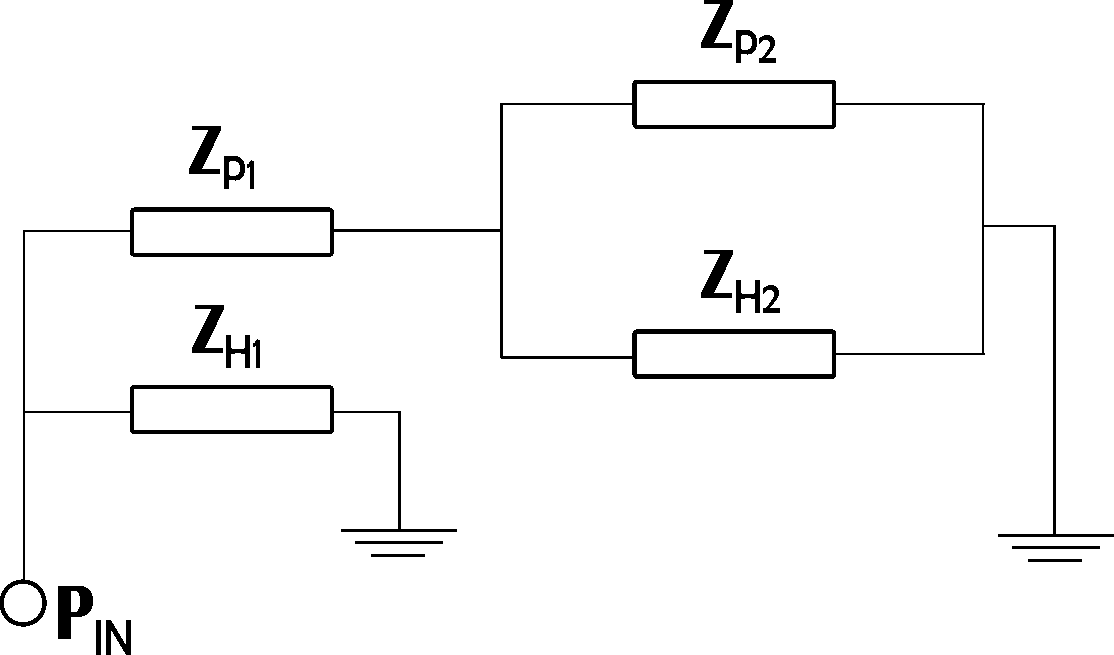
\includegraphics[width=0.7\textwidth]{twoholes.pdf}
	\caption{Electrical analog of the load impedance with two open holes. The subscripts $h_1$ and $p_1$ refer to the first hole and the section of the bore between the open holes, while $h_2$ and $p_2$ refer to the second hole and the terminating section of the pipe. The reference is the atmospheric pressure, while $P_{in}$ is the pressure at the end of the closed section of the tube.}
	\label{fig:holes}
\end{figure}

The situation is analogous when there are mutiple finger holes, albeit a little more complex. The radiation load at the end of the closed section of the tube will now include four components, arranged as in Fig. \ref{fig:holes}. The resulting load impedance will be $Z_r = Z_{h_1}\parallel\left(Z_{p_1} + Z_{h_2}\parallel Z_{p_2} \right)$. This gives us a new expression for the decrease in acoustic length of the bore:
\begin{align*}
	\delta &\approx D + D' + \Delta - \Delta'', \\
	\text{where } \Delta'' &= \frac{l(D+\Delta') }{(D'+\Delta') + \frac{lS_2}{S_h}} \\
\end{align*} 

The result for the distance between the two holes, solving for the frequency $f_2 = 440~\si{\hertz}$, is $D'= 3.69~\si{\centi\meter}$.

\section{Flue channel and mouth}
\subsection{Channel thickness}

Given the pressure difference $\Delta p$ between the player's mouth and the flue channel entrance, the flow velocity $U_j$ in the flue channel can be easily recovered from the Bernoulli equation:
\[
	\frac{1}{2} \rho_0 \left( v_2^2 - v_1^2 \right) = p_2 - p_1 \quad \Rightarrow \quad
	U_j = \sqrt{\frac{2\Delta p}{\rho_0}}
\]
where $v_2 = U_j$ is the jet velocity in the channel, $v_1 = 0$ is the air velocity in the player's mouth (assumed negligible) and $p_1$ and $p_2$ are the corresponding pressures.

Now, we know that the amplification of the jet perturbation is strongly dependent on the frequency of the acoustic field, and that it is strongest for frequencies around $0.3U_j / h$. This allows us to choose $h$ according to the desired spectral characteristics of the instrument: we can \textquote{tune} the channel thickness to maximize the perturbation amplification at a target spectral centroid $f_c$, choosing $ h = 0.3 U_j / f_c$.

In our particular case we can compute:
\begin{align*}
		&\Delta p = \SI{62}{\pascal},~ f_c = \SI{2}{\kilo\hertz},~ \rho_0 = \SI{1.2}{\kilogram\per\meter\cubed} &\longrightarrow \quad &\boxed{h = \SI{1.5}{\milli\metre}}\\
\end{align*}

The structure of the jet can be characterized using the Reynolds number:

$$ \mathrm{Re} = \frac{U_j h}{\nu} = 1033.3 $$

where $\nu = 1.5 \cdot 10^{-5}~ \si{\meter\squared\per\second}$ is the kinematic viscosity of the air. Typically, the transition between laminar and turbulent flow is considered to occur for values of Re in the range 2000-4000, so it is safe to say that we are dealing with a laminar flow at the channel exit, and it is expected to remain laminar for a short distance. Therefore, as long as $W$ isn't much larger than $h$, we expect the flow in the mouth to be laminar. 

\subsection{Boundary layer effects}
Of course the result for the flow velocity we found above is only valid at the center of the flow. Indeed, even if the fluid can be safely assumed to be frictionless in open space, the boundary conditions in a channel make the viscosity effects significant near the walls. There will be a thin layer extending from the boundary into the fluid where the velocity increases rapidly from zero to the value $U_j$: this is the so-called \emph{boundary layer}. The thickness of the boundary layer increases along the length of the channel: at position x along the channel it is:
$$ \delta(x) \approx \sqrt{\frac{\nu x}{U_j}}. $$
This means that for a channel length of 20 mm we get $\delta = \SI{0.17}{\milli\meter}$. Notice that $\delta/h = 0.11 < \frac{1}{2}$, so we can expect the Bernoulli approximation to hold reasonably well in the center of the channel.

\subsection{Dimensioning the length of the mouth}
We want to dimension the length of the mouth so that, under the blowing conditions described above, with all holes closed, we get a sound pressure level of 90 dB at the resonator foot.

To tackle this problem we are going to make a series of assumptions. The first one is that we can consider the bore as a lossless transmission line of length $L' = L + 0.3d_2$, so that at steady state the pressures at the foot and at the head differ only in phase. In this way, we can assume that the pressure at the head is equal in magnitude to the pressure at the foot, which gives us $p_{in} = 1.2017~\si{\pascal}$. This assumption allows us as well to compute the desired value of the flow injected into the resonator 

\end{document} 